


\newcommand{\FigHighLevel}{

\begin{figure}[ht]
    \centering
    % 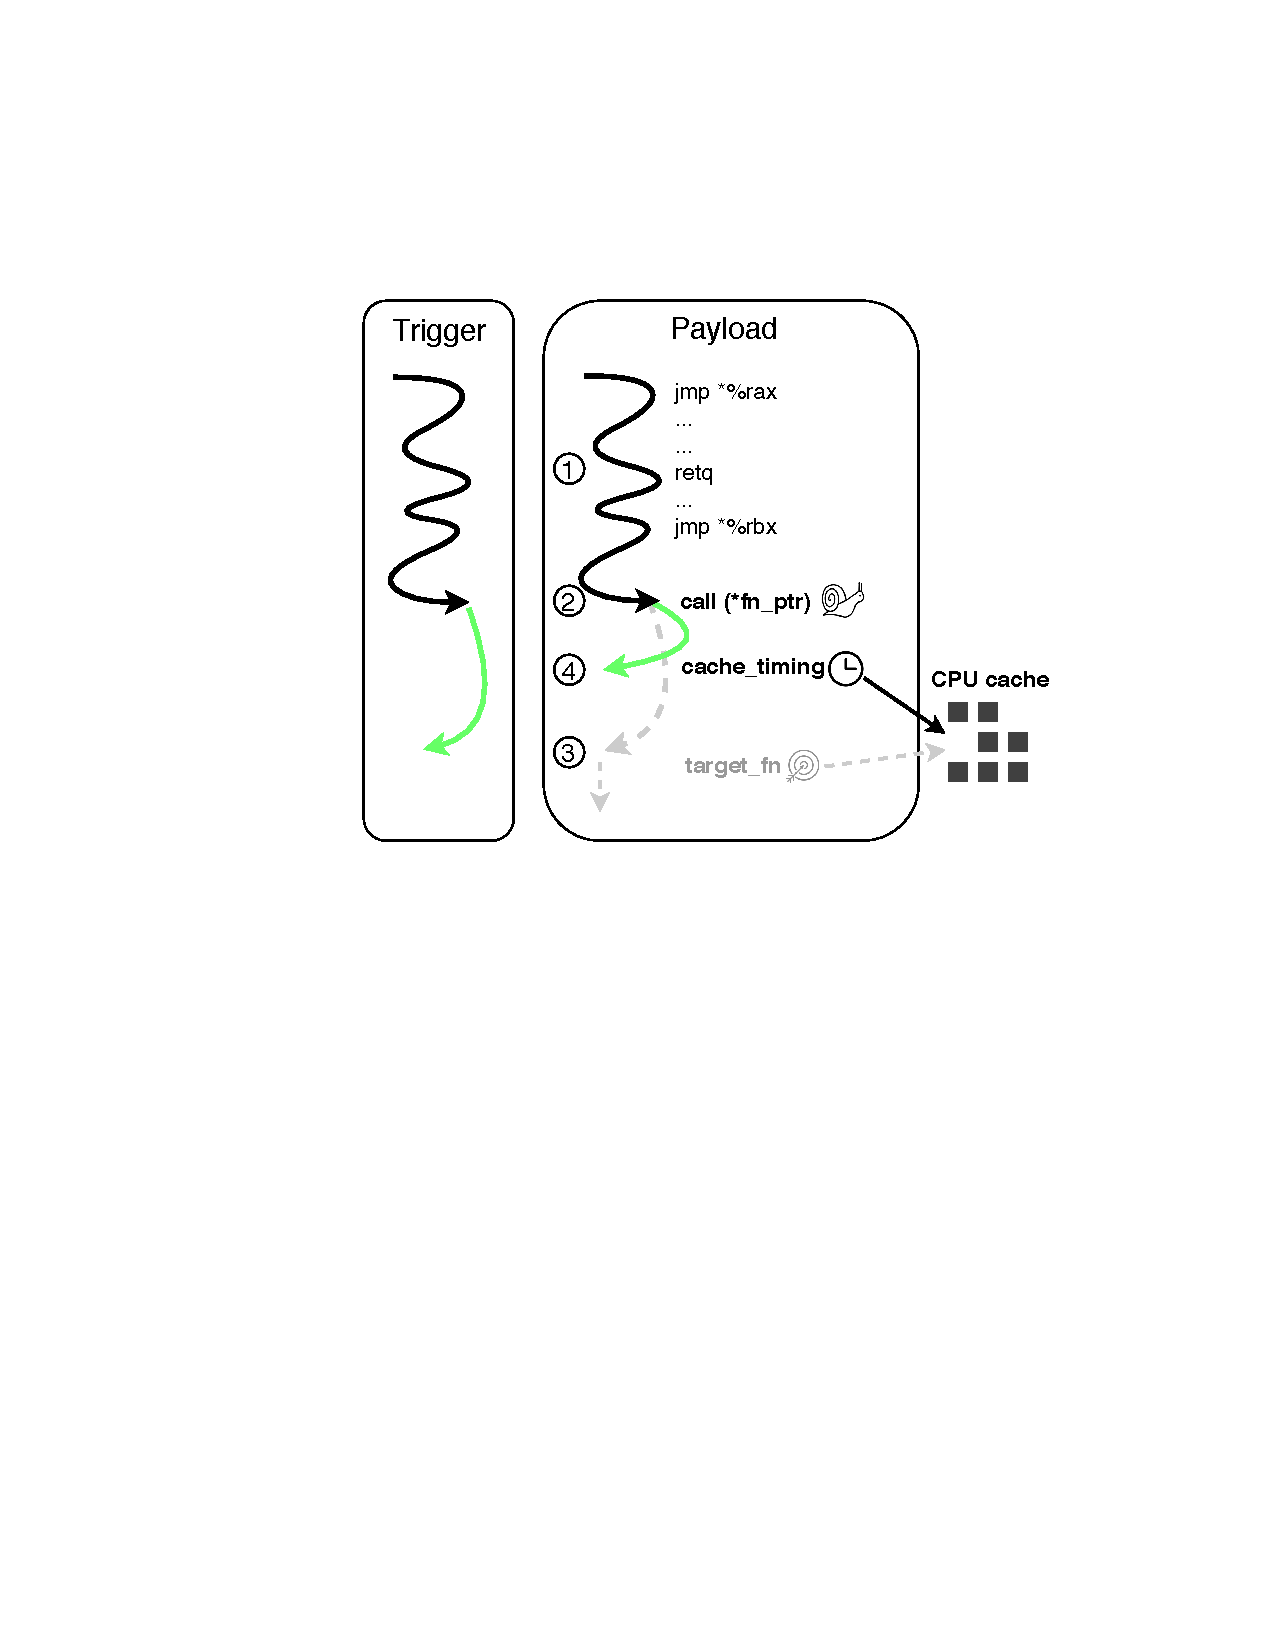
\includegraphics[clip, trim=6cm 13.5cm 3.8cm 5cm, width=0.9\linewidth]{figures/exspectre-high-level.pdf}
    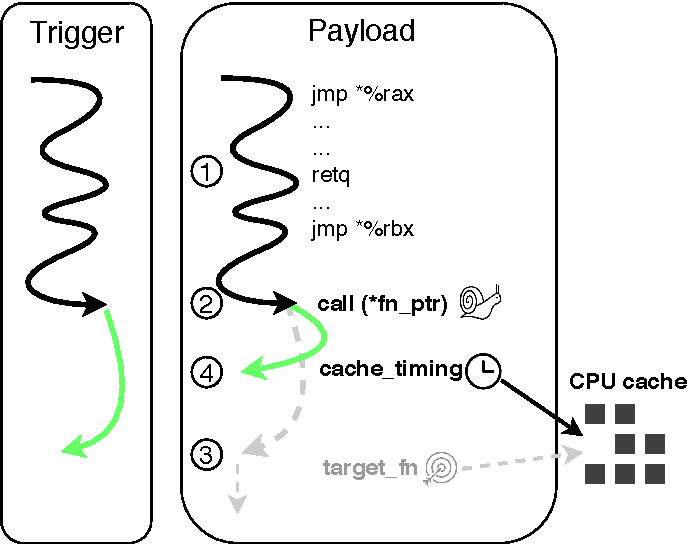
\includegraphics[width=0.9\linewidth]{figures/exspectre-high-level-trimmed.pdf}
    \caption{\textbf{\speculake}\,---\,%
    Both the Trigger and Payload binaries exhibit the same initial series of
    indirect jumps, shown in Step 1. The trigger program solely executes these
    jumps to (mis)train the branch predictor. In the Payload program
    \texttt{fn\_ptr} has been set to point to the \texttt{cache\_timing}
    function and flushed from cache. Thus at Step 2 the branch predictor
    mis-predicts the jump to \texttt{cache\_timing} and instead jumps to
    \texttt{target\_fn} as trained by the Trigger program (green line). 
    \texttt{target\_fn} then executes speculatively as shown in Step 3. 
    Eventually \texttt{fn\_ptr} is loaded from memory and this mis-jump is 
    recognized by the processor, directing computation to Step 4, the 
    \texttt{cache\_timing} function, which then computes which value was loaded 
    into cache speculatively.}


    \label{fig:high-level}

\end{figure}
}


\newcommand{\FigSpecMeasure}{
\begin{figure*}[t]
    \centering
        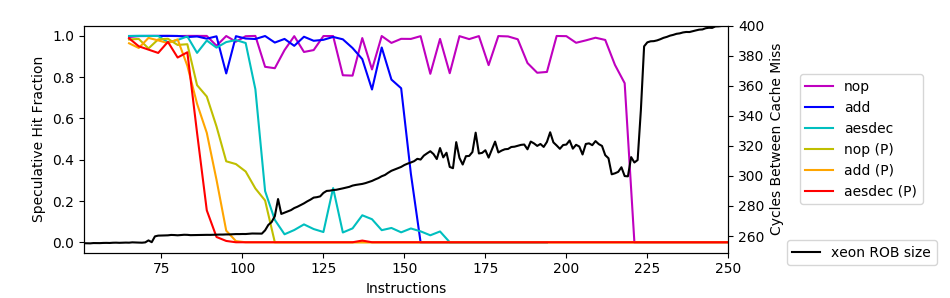
\includegraphics[width=0.9\textwidth]{figures/Speculative_measurements.png}
    \caption{The speculative primitive allows for a limited number of instructions
        to be completed speculatively, dependent on multiple factors. Trigger and 
        payload processes must share CPU resources as they must be performed on 
        the same hyperthread or associated parity hyperthreads. Processes on
        the parity hyperthreads (warm colors) denoted by (P) accomplish a 
        significantly lower number of instructions as compared with processes 
        on the same hyperthread (cool colors).}
    \label{fig:spec-capacity}
\end{figure*}
}


\newcommand{\FigCacheMiss}{
\begin{figure}[t]
    \centering
    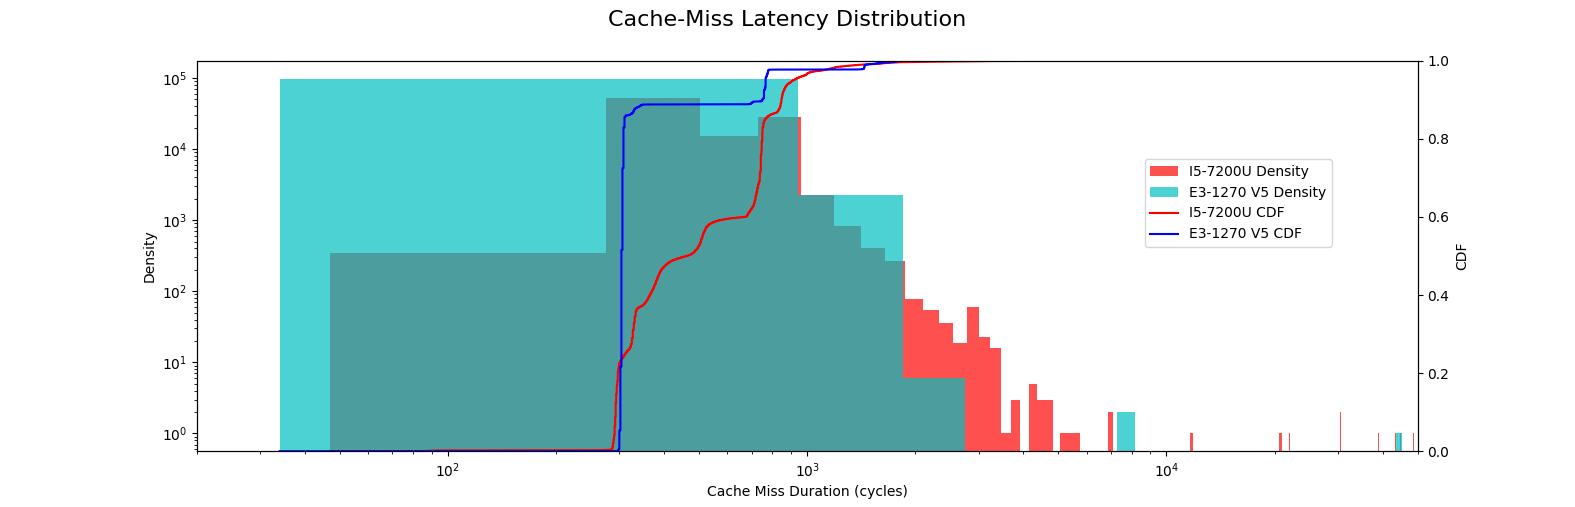
\includegraphics[width=0.5\textwidth]{figures/cache_miss_dist}
    \caption{The Cache Hit/Miss Latency Distribution of an Intel
        Xeon-1270. Measured by timing accesses to cached/uncached memory. 
        Typical cache miss resolution takes 6x longer than a cache hit.}
    \label{fig:cache-miss}
\end{figure}
}


\newcommand{\FigGeneralModel}{
\begin{figure}[t]
    \centering
        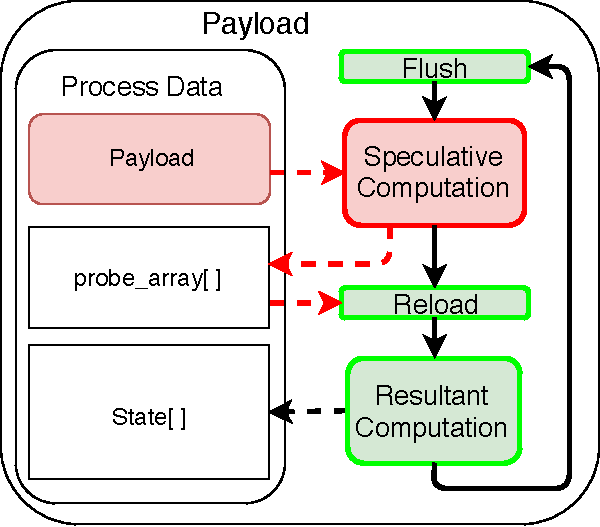
\includegraphics[width=0.4\textwidth]{figures/general_model.pdf}
    \caption{General model of speculative computation within the Payload 
        process when triggered. \textit{Speculative Computation} has read-only
        access to all memory within the process, and returns a result via a
        cache side channel (via the \texttt{probe\_array}).
        The process can subsequently make
        \textit{Resultant Computations} based on the value returned from
        the cache side channel to update the state of the process. }
    \label{fig:general_model}
\end{figure}
}


\newcommand{\FigSpecBandwidth}{
\begin{figure}[t]
    \centering
        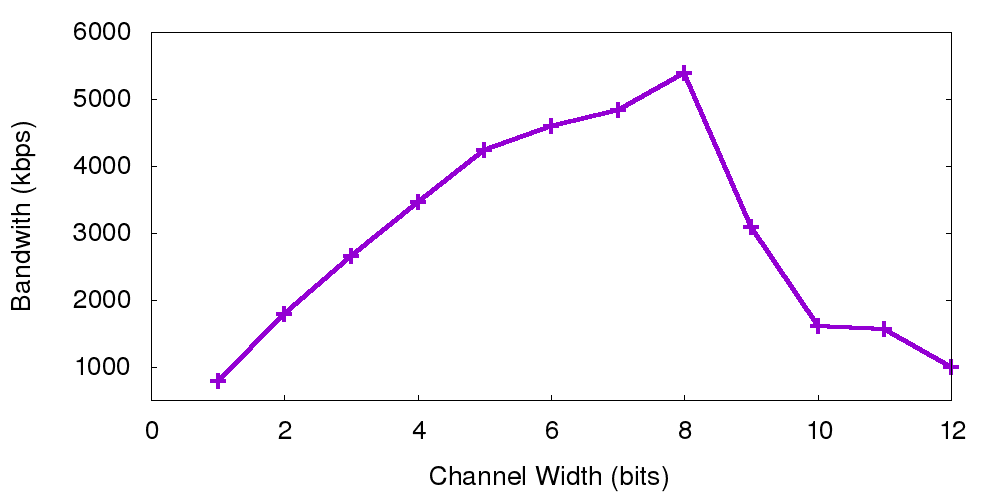
\includegraphics[width=0.5\textwidth]{figures/Speculative_bandwidth}
    \caption{Speculative Bandwidth---Using the speculative primitive 
        1KB of data can be decrypted and exfiltrated at a speed between 5 and 6 kbps
        from the speculative world with 20 iterations per
        round for guaranteed correctness.  Varying the width of the channel 
        results in competing performance factors -- decreasing the 
        number of loops vs decreased size of the probe space.}
    \label{fig:spec_bandwidth}
\end{figure}
}



\newcommand{\FigSpasmModel}{
\begin{figure}[b]
    \centering
        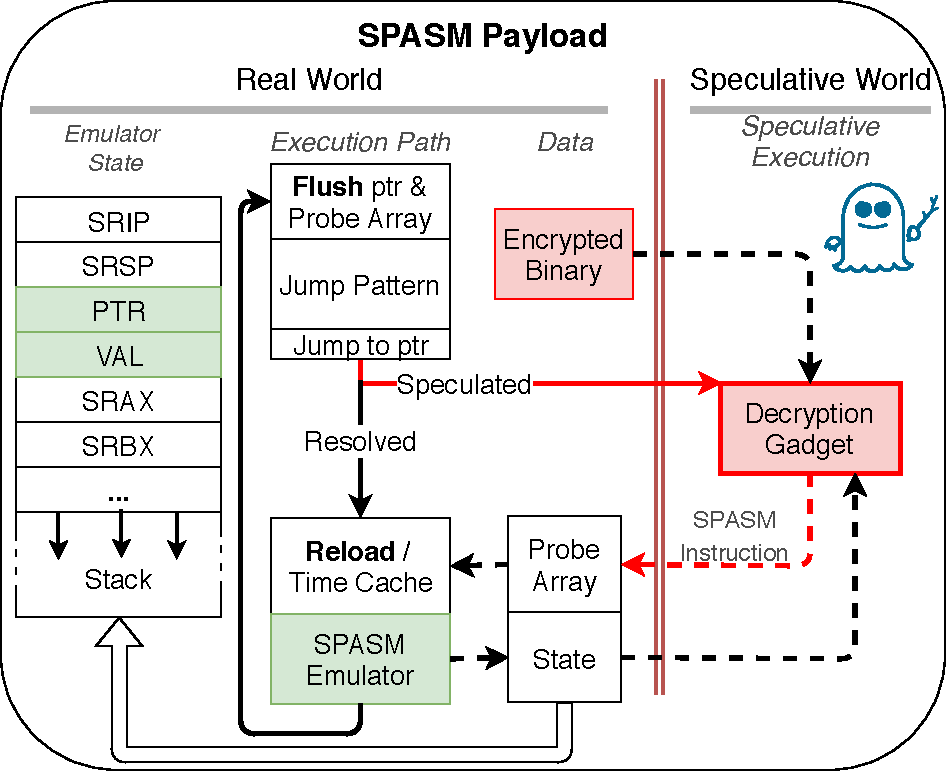
\includegraphics[width=0.46\textwidth]{figures/spasm_model.pdf}
    \caption{This diagram demonstrates the control flow of a \speculake application
        making use of the decryption gadget and emulation. An encrypted SPASM binary 
        stored in dead code or data accessible to \textit{Speculative Computation} 
        is decrypted  and then returned through the primitive. The 
        \textit{Resultant Computation} performs the SPASM emulation to update the 
        process state before the next instruction is decrypted.}
    \label{fig:spasm_model}
\end{figure}
}

\newcommand{\FigTuringSuccess}{
\begin{figure}[t]
    \centering
        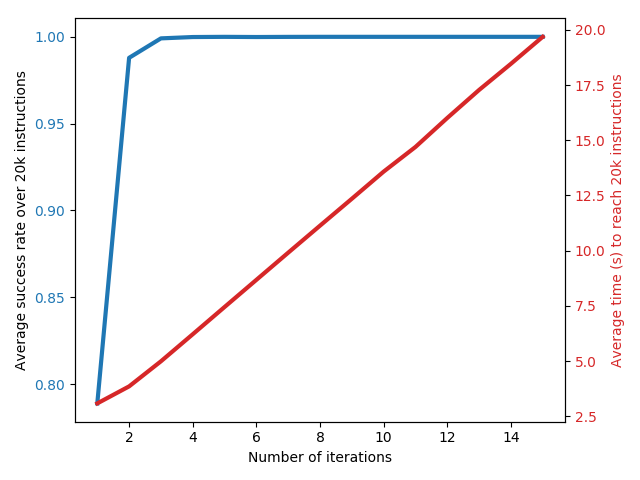
\includegraphics[width=0.46\textwidth]{figures/SuccessAndTime}

    \caption{The number of instructions and error rate of a the 5-state Busy
            Beaver configuration were measured as a function of how many (redundant) iterations into
    the speculative world were performed. As expected, the amount of time to
    complete a million instructions is a linear function of how many
    indirect calls into the speculative world we take. Additionally we see that
    it only requires using 10 speculative calls per instruction to achieve a
    very low number of errors in reaching a million instructions, making 10-20
    iterations an attractive choice for most applications.}

    \label{fig:turing_success}
\end{figure}
}
